\chapter{Komponenten}
\section{Filter}
\subsection{Tiefpassfilter}
\begin{figure}[H]
    \centering
    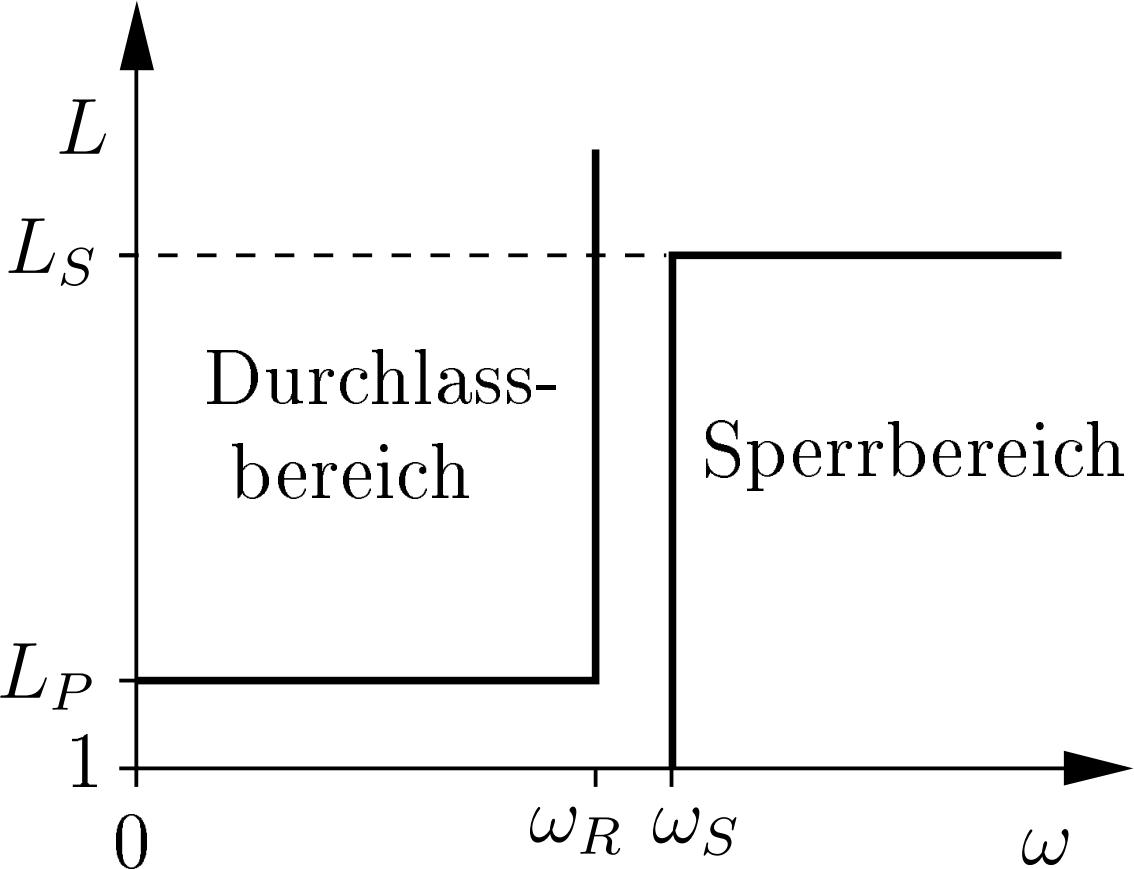
\includegraphics[width=.5\textwidth]{images/tiefpass.png}
\end{figure}
\begin{description}
    \item[Filterkoeffizienten] $g_i$ bestimmen Dämpfungsverlauf
    \item[Referenzwiderstand] $= R_0$ Quellenwiderstand
    \item[Durchlassband-Eckkreisfrequenz] $\omega_R$: Frequenz, bis zu der maximal die
        \emph{Durchlass- / Passband-Dämpfung $L_P$} gilt
    \item[Sperrkreisfrequenz] $\omega_S$: Frequenz, ab der minimal die
        \emph{Sperrband-Dämpfung $L_S$} gilt.
\end{description}
Mit den Filterkoeffizienten $g_i$ lassen sich die Bauteilwerte ausrechnen:
\begin{equation}
    L_i = \frac{R_0g_i}{\omega_R}
\end{equation}
\begin{equation}
    C_i = \frac{g_i}{R_0\omega_R}
\end{equation}
Für die Last gilt wenn die letzte Reaktanz ein Parallelelement ist:
\begin{equation}
    R_{n+1} = g_{n+1} R_0
\end{equation}
Und wenn die letzte Reaktanz ein Serienelement ist:
\begin{equation}
    R_{n+1} = \frac{R_0}{g_{n+1}}
\end{equation}

Mit der normierten Kreisfrequenz $\omega' = \frac{\omega}{\omega_R}$ gilt unabhängig vom
Filterprototyp die \emph{Feldtkellersche Gleichung} für die Dämpfung $L$:
\begin{equation}
    L(j\omega') = 1 + \abs{K(j\omega')}^2
\end{equation}
wobei die \emph{charakteristische Funktion $K()$} abhängig vom Filterprototyp ist.

\subsubsection{Butterworth}
Der Butterworth Filter wird als \emph{maximalflaches Filter} bezeichnet.
Bei vorgegebenen $\omega_P, \omega_S, L_P, L_S$ kann die minimale Ordnung berechnet werden.
Ein Butterworth Filter mit Filtergrad $n$ besitzt $n$ Reaktanzen, die Filterkoeffizienten berechnen
sich durch:
\begin{align}
    g_0 &= 1\\
    g_k &= 2 \sin\left( \frac{(2k-1)\pi}{2n} \right)\\
    g_{n+1} &= 1
\end{align}
Mit steigender Filterordnung geht die Dämpfung gegen $20n\si{\decibel}$ pro Dekade.

\subsubsection{Tschebyschow}
Der Tschebyschow Filter wird als \emph{equal ripple filter} bezeichnet aufgrund der regelmäßigen
Schwankung der Dämpfung im Durchlassbereich. Typische maximale Dämpfungen im Durchlassbereich
sind \SI{0.01}{\decibel} - \SI{0.5}{\decibel}.
Mit steigender Filterordnung geht die Dämpfung gegen $20n\si{\decibel}$ pro Dekade.
Die Anzahl der Reaktanzen ist wieder $n$, was auch der Anzahl der Kontaktpunkte der Dämpfungskurve
mit der Frequenzachse entspricht.
Ein Vorteil gegenüber Butterworth ist die scheinbar höhere Steilheit der Filterflanke, tatsächlich
setzt diese aber nur früher ein. Nachteil ist die Welligkeit und die höhere Gruppenlaufzeit.

\todo{Transformation zu HP/BP/BS}


\subsection{Frequenzvervielfacher, Mischer}
Zur Implementierung eines Mischers werden nichtlineare Bauelemente wie Dioden verwendet.
Nach Taylorreihenentwicklung der Kennlinie und Anwendung von Additionstheoremen ergeben sich
Mischfrequenzen. Insbesondere bei anlegen additiv überlagerter Eingangssignale die Summe und Differenz
der beiden Frequenzen. Grundlegend treten alle Frequenzen
$f_i = \abs{mf_\text{LO}+nf_S}$ mit $m,n\in\mathbb{Z}\setminus\{0\}$
